\documentclass[12pt]{article}
\usepackage[utf8]{inputenc}
\usepackage[a4paper,top=20mm]{geometry}
\usepackage{hyperref}
\usepackage{setspace}
\usepackage{amsfonts}
\usepackage{amsthm}
\usepackage{graphics}
\usepackage{tikz}
\graphicspath{ {./images/} }
\usepackage{graphicx}
\usepackage{amssymb}
\usepackage{amsmath}
\usepackage{parskip}

\theoremstyle{definition}
\newtheorem{definition}{Definition}

\newtheorem{theorem}{Theorem}
\newtheorem{corollary}{Corollary}[theorem]
\newtheorem{lemma}[theorem]{Lemma}

\newcommand\ddfrac[2]{\frac{\displaystyle #1}{\displaystyle #2}}
\newcommand*\circled[1]{\tikz[baseline=(char.base)]{
            \node[shape=circle,draw,inner sep=2pt] (char) {#1};}}
\DeclareMathOperator{\Deg}{deg}
\title{ZPC-26}
\author{Farhan, Raunak, Ishaan, Mudit}
\date{\today}
\doublespacing
\begin{document}

\maketitle
\title{\textbf{\underline{\fontsize{18}{12}\selectfont Instructions}}}\\
Please read the following instructions carefully before proceeding further:\\
\begin{enumerate}
\item The test is of 2 hours. It will end \textit{sharp} at \textbf{8:00 pm}.
\item Relevant reading material for all the questions has been provided in the document itself.
\item If you are stuck on a question that you cannot figure out, move on. Nothing good ever comes out of being hung up on something.
\item Please feel free to contact the invigilators in case of any queries.
\item We will provide hints to questions in the last hour, depending on the participation and responses.
\item All the best. GL HF :)\\
\end{enumerate}
\bigskip
\maketitle
\newpage
\title{\begin{center}\textbf{\underline{\fontsize{16}{12}\selectfont HOMOTHETY}}\end{center}}
\section{Introduction}
\textbf{Homothety} is one of the most interesting things in Euclidean geometry. Before formally defining homothety, we give some examples to give the reader a feeling of what homothety is.

Speaking in simpler terms, Homothety is nothing but a dilation of a geometric figure about a center. You can think of Homothety as scaling a mathematical figure about a point. For example, see the following figure:

\begin{center}
    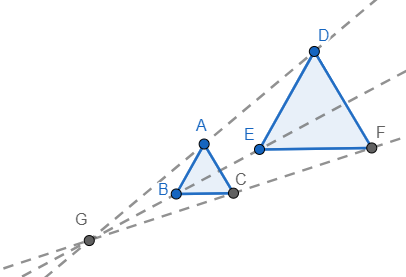
\includegraphics[]{images/Screenshot 2023-03-16 233654.png}
\end{center}
The above figure can be called a homothety from $\Delta ABC$ to $\Delta DEF$ about point $G$. It can also be seen as a homothety from $\Delta DEF$ to $\Delta ABC$ about point $G$.

That gives you the basic intuition of Homothety. Now, we move to the formal definition.


\section{Formal Definition of Homothety}
From the previous section, we understand that a homothety or dilation or central similarity is a special type of similarity,
in which a figure is dilated from a center. It is just equivalent to scaling a figure about a center. The formal definition of Homothety is as follows:
\begin{definition}[Homothety]
As homothety $h$ is a geometric transformation defined by a center $O$ and a real number $k$. It sends a point $P$ to another point $h(P)$, multiplying the distance from $O$ by $k$.
The number $k$ is called the scale factor of the homothety.
\end{definition}
 For example, the below figure shows a homothety $h$ that maps the points of a triangle $\Delta ABC$ to $\Delta h(A)h(B)h(C)$ about the point $O$ and scales it by a factor of $k=3$.
 \begin{center}
     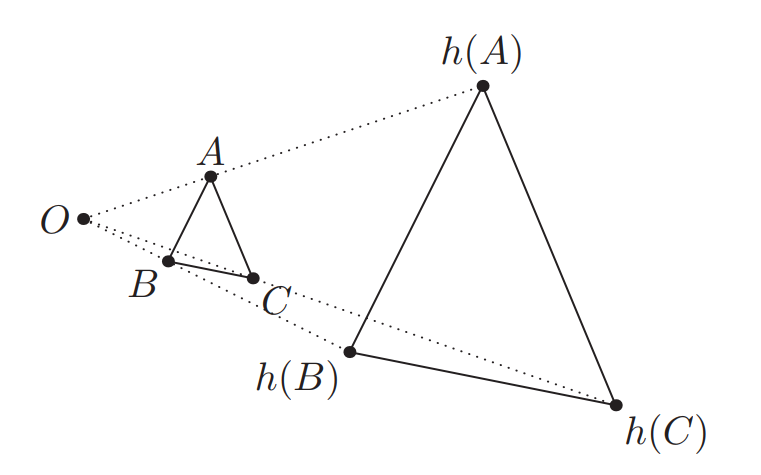
\includegraphics[scale=0.7]{images/zpcpic2.png}
 \end{center}
Note that on changing the center $O$ the homothety can completely change. Also, by changing the factor $k$, the homothety changes. It is important to note that $k$ can be negative, in which case we have a negative homothety and the two figures lie on the opposite sides of the center $O$. The following figure shows a negative Homothety.

\begin{center}
    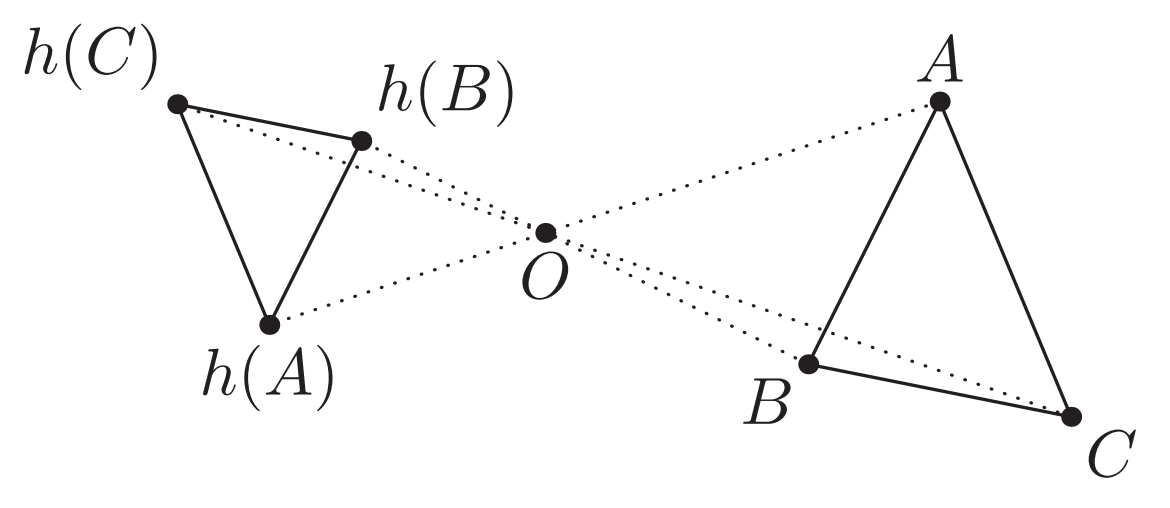
\includegraphics[scale=0.5]{images/zpcpic3.png}
\end{center}

Homothety preserves many things, including but not limited to tangency, angles, circles, and so on. They do not preserve length, but they work well enough: the lengths are simply all multiplied by k.

\section{More about Homothety}
Given non-congruent parallel segments $\overline{AB}$ and $\overline{XY}$ (what happens if $\overline{AB} = \overline{XY}$ ?), we can consider the intersection point O of lines $\overline{AX}$ and $\overline{BY}$ . This is the center of a homothety sending one segment to the other. (As is the intersection of lines $\overline{AY}$ and $\overline{BX}$—one of these is negative.) As a result, parallel lines are often indicators of homotheties. It is useful for proving collinearity, concurrency, determining ratios, and constructing points. 

Any homothety satisfies the following properties:
\begin{enumerate}
    \item Under a homothety, parallel lines map onto parallel lines.
    \item Homothety preserves angles.
    \item Homothety preserves orientation.
    \item Every homothety has an inverse.(Homothety with factor $k$ will be cacelled by a homothety of factor $\displaystyle\frac{1}{k}$) 
    \item Successive application of two homotheties with factors $k_1$ and $k_2$ can be thought as a homothety with factor $k_1k_2$. This is called the multiplication of homotheties. Note that this multiplication of homotheties is not commutative because even though the resulting homotheties will have the same factors but they my have different positions in space.
    \item Product of homotheties is not associative.
\end{enumerate}









\newpage
\maketitle
\title{\begin{center}\textbf{\underline{\fontsize{18}{12}\selectfont PROBLEMS}}\end{center}}
\begin{itemize}
    \item The questions here are all subjective, and will be graded on how well you can convince the checker of the mathematical rigour of your solution.
    \item The corresponding points of each question are mentioned with it. Do note that the points may or may not be proportionate to the relative difficulty of the question.
    \item The number of problems presented is much more than what is humanly possible to solve in the given time frame. Hence, prioritise correctness and rigour over number of problems solved.
    \item Note that any significant conclusion derived in the right direction to solve the problem may fetch you some points, so try to attempt all questions.
\end{itemize}
\bigskip
\bigskip
\bigskip
\begin{enumerate}
    \item For every two non-intersecting circles, prove that there exists at least 2 homotheties mapping one to each other (1 point)\\

    \item Let $ABCD$ be a parallelogram and let $E$ be a point on the side $AB$ for which $AE:EB= 2 : 1$. Suppose that $BD$ and $CE$ intersect at $F$. Determine $BF:FD$ (2 points)\\

    \item Prove Pythagoras' theorem using homotheties (2 points)\\
    
    \item Let the incircle of triangle $PQR$ touch side $QR$ at $D$, and let $DT$ be a diameter of the circle. If line $pT$ meets $qr$ at $X$, then $QD = RX$ (3 points)\\
    
    \item Let $H$ be the orthocentre of triangle $ABC$, then prove that the midpoints of the sides, the pedal points (feet of the altitudes) and the midpoints of $AH$, $BH$, $CH$ all lie on a common circle (3 points)\\
    
    \item $ABC$ and $A'B'C$ are similarly oriented equilateral (differ only by a rotation) triangles intersecting only at $C$;$P$,$Q$,$R$ are the respective midpoints of $AB'$, $BC$, $A'C$. Prove that triangle $PQR$ is equilateral (4 points)\\
    
    \item Triangle $ABC$ has orthocenter $H$, incenter $I$ and circumcenter $O$. Let $K$ be the point where the incircle touches $BC$. If $IO\parallel BC$, then prove that $AO\parallel HK$ (5 points)\\

\end{enumerate}
$$\square \square \square \square \square \square \square \square \square \square \square \square \square \square \square $$
\end{document}